\documentclass[noinstructornotes]{ximera}
%handout:  for handout version with no solutions or instructor notes
%handout,instructornotes:  for instructor version with just problems and notes, no solutions
%noinstructornotes:  shows only problem and solutions

%% handout
%% space
%% newpage
%% numbers
%% nooutcomes

%I added the commands here so that I would't have to keep looking them up
%\newcommand{\RR}{\mathbb R}
%\renewcommand{\d}{\,d}
%\newcommand{\dd}[2][]{\frac{d #1}{d #2}}
%\renewcommand{\l}{\ell}
%\newcommand{\ddx}{\frac{d}{dx}}
%\everymath{\displaystyle}
%\newcommand{\dfn}{\textbf}
%\newcommand{\eval}[1]{\bigg[ #1 \bigg]}

%\begin{image}
%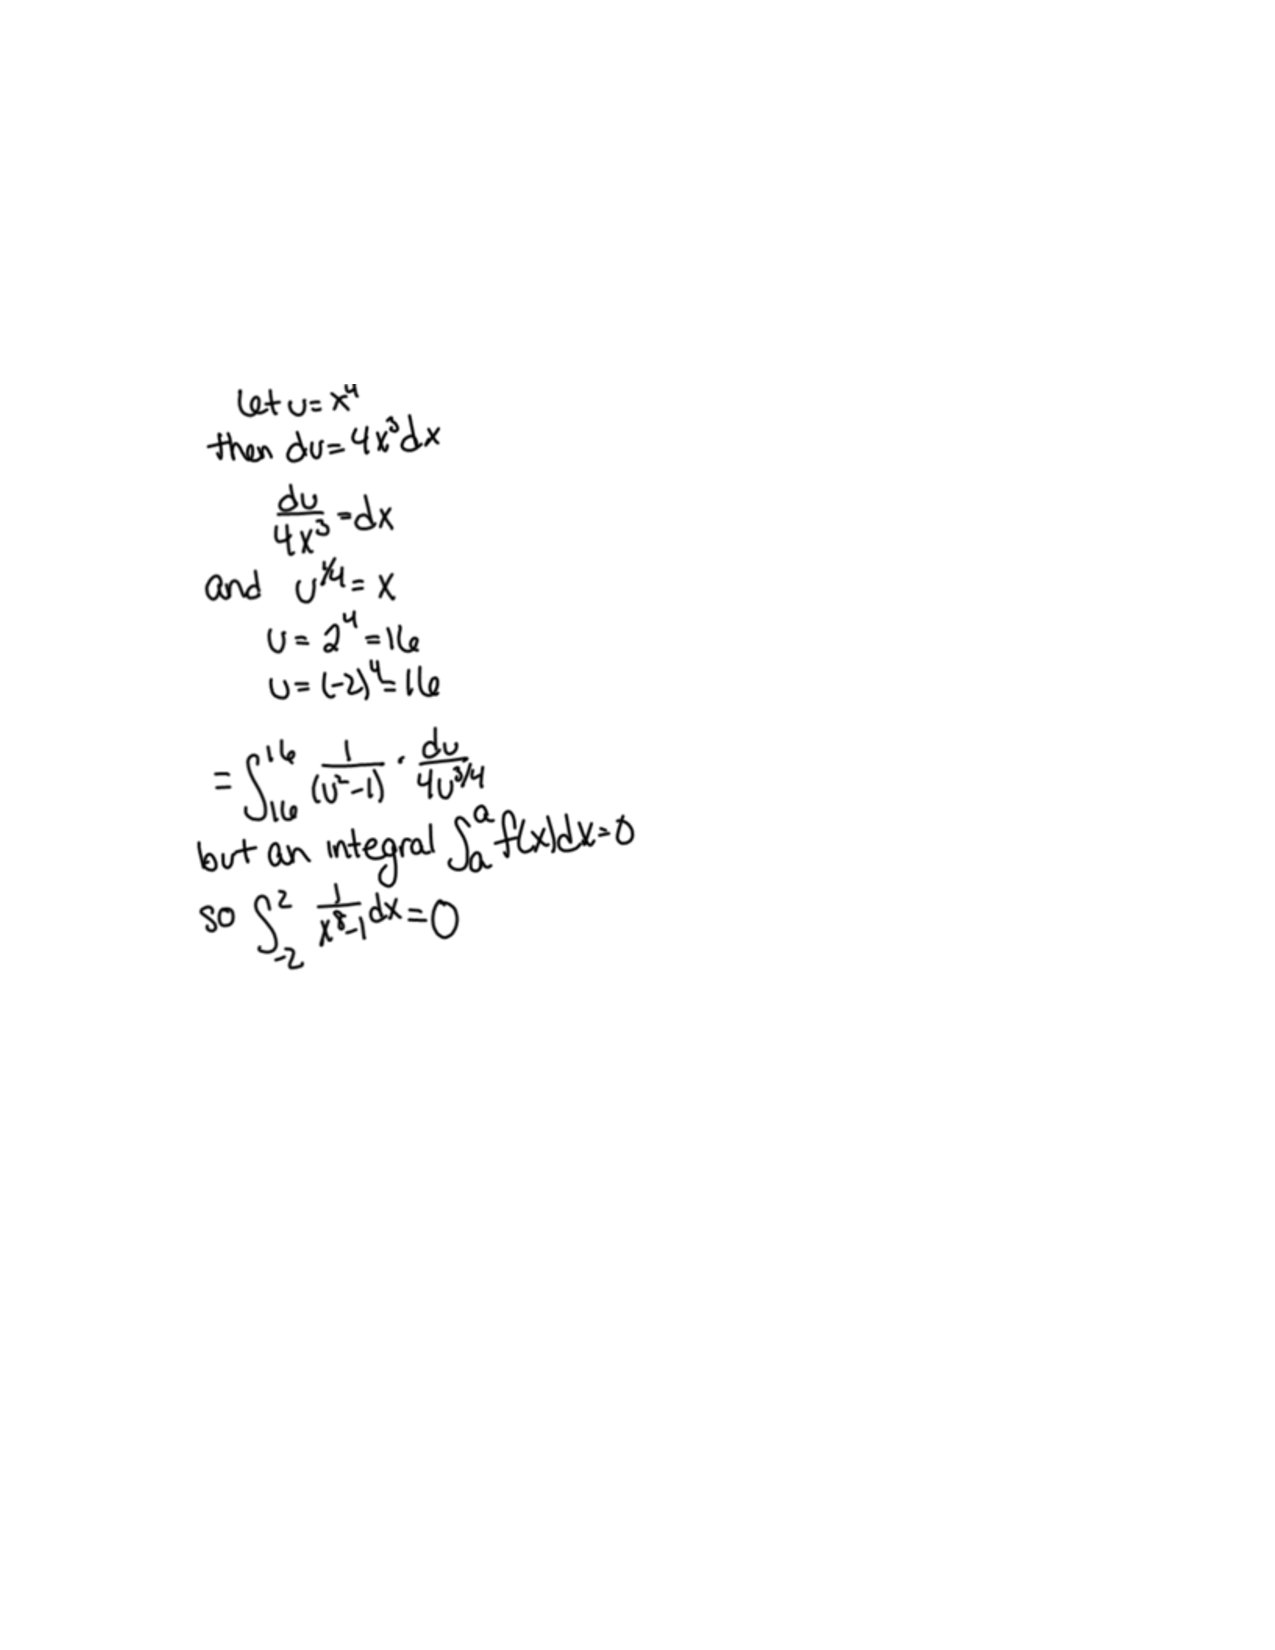
\includegraphics[trim= 170 420 250 180]{Figure1.pdf}
%\end{image}

%add a ``.'' below when used in a specific directory.
\newcommand{\RR}{\mathbb R}
\renewcommand{\d}{\,d}
\newcommand{\dd}[2][]{\frac{d #1}{d #2}}
\renewcommand{\l}{\ell}
\newcommand{\ddx}{\frac{d}{dx}}
\newcommand{\dfn}{\textbf}
\newcommand{\eval}[1]{\bigg[ #1 \bigg]}

\usepackage{multicol}

\renewenvironment{freeResponse}{
\ifhandout\setbox0\vbox\bgroup\else
\begin{trivlist}\item[\hskip \labelsep\bfseries Solution:\hspace{2ex}]
\fi}
{\ifhandout\egroup\else
\end{trivlist}
\fi} %% we can turn off input when making a master document


\title{Section 9.4: Divergence and Integral Tests and Conceptual Questions}  

\begin{document}
\begin{abstract}		\end{abstract}
\maketitle

\section{Warm-Up}
\begin{problem} Suppose $\displaystyle \sum_{k=1}^{\infty} a_k$ is an infinite series.
\begin{itemize}

\item[A.] If $\displaystyle \lim_{k \rightarrow \infty} a_k = 0$, does $\displaystyle \sum_{k=1}^{\infty} a_k$ have to converge?
\begin{freeResponse}
No; consider the harmonic series $\displaystyle \sum_{k=1}^{\infty} \dfrac{1}{k}$.  Here $a_k = \dfrac{1}{k}$, so $\displaystyle \lim_{k \rightarrow \infty} a_k = 0$, but the series diverges!
\end{freeResponse}

\item[B.] If $\displaystyle \sum_{k=1}^{\infty} a_k$ converges, does $\displaystyle \lim_{k \rightarrow \infty} a_k = 0$ necessarily?
\begin{freeResponse}
Yes; if $\displaystyle \lim_{k \rightarrow \infty} a_k \neq 0$, the divergence test guarantees that 
$\displaystyle \sum_{k=1}^{\infty} a_k$ diverges.  Since we know the series converges by assumption, we must have $\displaystyle \lim_{k \rightarrow \infty} a_k = 0$!
\end{freeResponse}
\end{itemize}
\end{problem}

\section{Group Work}

\begin{problem}
Suppose $\displaystyle\{a_n\}_{n \geq 1}$ is a sequence and $\displaystyle \sum^{\infty}_{n= 1} a_n$ converges to $L>0$.  Let $s_n =\displaystyle  \sum^n_{k=1} a_k$.  Circle all of the statements that \emph{MUST} be true. 

\begin{tabular}{lll}
A. $\displaystyle \lim_{n \rightarrow \infty} a_n = L$ \qquad  \qquad  & B. $\displaystyle \lim_{n \rightarrow \infty} a_n = 0$ \qquad  \qquad  & C. $\displaystyle \lim_{n \rightarrow \infty} s_n = 0$   \\ [5ex] 
D. $\displaystyle \lim_{n \rightarrow \infty} s_n = L$ \qquad   \qquad  &E.  $\displaystyle \sum^{\infty}_{n=1} s_n$ MUST diverge. \qquad  \qquad  &F. $\displaystyle \sum^{\infty}_{n=1} (a_n+1) = L+1$ \\
\end{tabular}

\hspace{.5mm} G. The divergence test tells us $\displaystyle \sum^{\infty}_{n= 1} a_n$ converges to $L$.


\begin{freeResponse}

\begin{itemize}
\item[A.] \textbf{False} \\ Since $\displaystyle\{a_n\}_{n \geq 1} = L$, $\displaystyle\{a_n\}_{n \geq 1}$ is a \emph{convergent} series, so $\displaystyle \lim_{n \rightarrow \infty} a_n = 0$.  Since $L>0$, there is no way that $\displaystyle \lim_{n \rightarrow \infty} a_n = L$.


\item[B.] \textbf{True} \\ If $\displaystyle \lim_{n \rightarrow \infty} a_n \neq 0$, the divergence test implies $\displaystyle \sum^{\infty}_{n= 1} a_n$ diverges!  Anytime a series $\displaystyle \sum^{\infty}_{n= 1} a_n$ converges, it MUST be true that $\displaystyle \lim_{n \rightarrow \infty} a_n = 0$. 

\item[C.] \textbf{False} \\ $\displaystyle \lim_{n \rightarrow \infty} s_n = \lim_{n \rightarrow \infty} \displaystyle  \sum^n_{k=1} a_k = \displaystyle \sum^{\infty}_{n= 1} a_n = L>0 $ 

\item[D.] \textbf{True} \\ Some essential facts are:
\begin{itemize}
\item $\displaystyle \sum^{\infty}_{n= 1} a_n$ converges iff $\displaystyle \lim_{n \rightarrow \infty} s_n = \lim_{n \rightarrow \infty} \displaystyle  \sum^n_{k=1} a_k$ exists

\item When $\displaystyle \lim_{n\rightarrow \infty} s_n$ does exist, $\displaystyle \displaystyle \sum^{\infty}_{n= 1} a_n = \lim_{n \rightarrow \infty} s_n$.  


\item The series $\displaystyle \sum^{\infty}_{n= 1} a_n$ likewise diverges iff the $\displaystyle \lim_{n\rightarrow \infty} s_n$ does not exist.
\end{itemize}
Here, we are given $\displaystyle \sum^{\infty}_{n= 1} a_n$ converges to $L>0$, which tells us immediately that $\displaystyle \lim_{n\rightarrow \infty} s_n = L$.


\item[E.] \textbf{True} \\ Since $\displaystyle \lim_{n\rightarrow \infty} s_n = L \neq 0$, the divergence test tells us immediately that $\displaystyle \sum^{\infty}_{n=1} s_n$ MUST diverge.

\item[F.] \textbf{False} \\ Since $\displaystyle \sum^{\infty}_{n=1} a_n$ converges, $\displaystyle \lim_{n \rightarrow \infty} a_n = 0$.  Thus, $\displaystyle \lim_{n \rightarrow \infty} (a_n+1) = 1$, and the divergence test immediately tells us that  $\displaystyle \sum^{\infty}_{n=1} (a_n+1)$ MUST diverge!

\item[G.] \textbf{False} \\ The divergence test \emph{NEVER} can be used to conclude that a series converges! 

\vspace{3mm}


\end{itemize}
\end{freeResponse}
\end{problem}




%problem 1
\begin{problem}
For each of the following, answer {\bf True} or {\bf False}, and explain why.
	\begin{enumerate}
	
	\item  If $\sum_{n=0}^\infty a_n$ converges, then $\sum_{n=0}^\infty (a_n + 0.001)$ converges.
	
	\item  Since $\int_1^\infty x \sin(\pi x) \d x$ diverges then, by the Integral Test, $\sum_{n=0}^\infty n \sin(\pi n)$ diverges.
	
	\item  Since $\int_1^\infty \frac{1}{x^2} \d x = 1$ then, by the Integral Test, $\sum_{k=1}^\infty \frac{1}{k^2} = 1$.  
	
	\end{enumerate}
	
	\begin{freeResponse}
		\begin{enumerate}
		
		\item  {\bf False}
		
		Since $\sum_{n=0}^\infty a_n$ converges, we know that $\lim_{n \to \infty} a_n = 0$.  
		But then 
			\[
			\lim_{n \to \infty} (a_n + 0.0001) = 0.0001 \neq 0
			\]
		and so $\sum_{n=0}^\infty (a_n + 0.001)$ diverges by the Divergence Test.
		
		
		
		\item  {\bf False}
		
		The Integral Test only holds for positive, decreasing functions.  
		The function $f(x)= x \sin(\pi x)$ is not always positive, nor is it always decreasing.  
		So the Integral Test does not apply here.
		
		This problem is simpler than that though.  
		Since $\sin(\pi n) = 0$ for all integers $n$, we have that $\sum_{n=0}^\infty n \sin(\pi n) = 0$.
		
		
		
		\item  {\bf False}
		
		The Integral Test tells us that $\sum_{k=1}^\infty \frac{1}{k^2}$ converges, but it does {\bf not} give us the sum (this sum is actually $\frac{\pi^2}{6}$).  
		
		\end{enumerate}
	\end{freeResponse}
	
\end{problem}

\begin{instructorNotes}
For part (b) we need $f(x)$ to be a decreasing function for the Integral Test to (necessarily) hold.
All groups should do all of the parts.
\end{instructorNotes}







%problem 2
\begin{problem}
Assume $\sum_{k=0}^\infty a_k =L$ and $b_k = 8$ for all $k$. 
	\begin{enumerate}
	
	\item  What is $\lim_{k \to \infty} (a_k + b_k)$?
	
	\item  What is $\lim_{k \to \infty} \sum_{n=0}^k (a_n + b_n)$?
	
	\item  What is $\lim_{k \to \infty} \sum_{n=0}^k (a_{n+1} - a_n)$?
	
	\end{enumerate}
	
	\begin{freeResponse}
		\begin{enumerate}
	
		\item  Since $\sum_{k=0}^\infty a_k$ converges, we know that $\lim_{k \to \infty} a_k = 0$.  
		Therefore,
			\[
			\lim_{k \to \infty} (a_k + b_k) = 0 + 8 = \boxed{8}.
			\]
	
		\item  Since $\lim_{n \to \infty} (a_n + b_n) = 8$, the series $\sum_{n=0}^\infty (a_n + b_n)$ diverges by the Divergence Test.  
		But $\lim_{k \to \infty}  \sum_{n=0}^k (a_n + b_n) = \sum_{n=0}^\infty (a_n + b_n)$.  
		Thus
			\[
			\lim_{k \to \infty}  \sum_{n=0}^k (a_n + b_n) = \sum_{n=0}^\infty (a_n + b_n) = \boxed{\infty}.
			\]
	
		\item  Let $S_k = \sum_{n=0}^k (a_{n+1} - a_n)$ (and recall that $\{ S_k \}$ is the {\it sequence of partial sums}).
		Then
			\begin{align*}
			S_k &= \sum_{n=0}^k (a_{n+1} - a_n)  \\
			&= (a_1 - a_0) + (a_2 - a_1) + (a_3 - a_2) + \hdots + (a_k - a_{k-1}) + (a_{k+1} - a_k)  \\
			&= a_{k+1} - a_0.
			\end{align*}
		Thus,
			\[
			\lim_{k \to \infty} \sum_{n=0}^k (a_{n+1} - a_n) = \lim_{k \to \infty} S_k = \lim_{k \to \infty} a_{k+1} - a_0 = \boxed{-a_0}.
			\]
	
		\end{enumerate}
	\end{freeResponse}
		
\end{problem}

\begin{instructorNotes}
This question was adapted from midterm \#2 in Spring 2013.  
Students had difficulty distinguishing between a question dealing with sequences vs. a question dealing with series.
\end{instructorNotes}





%Root and Ratio Test Problem
%problem 1
\begin{problem}
Determine if the following series converge or diverge.
	\begin{enumerate}
%	
%	\item  $\sum_{n=1}^\infty \frac{(7n+1)^2 \cdot 2^n}{5^n}$
%	
%	\item  $\sum_{n=1}^\infty a_n$, where $a_{n+1} = \frac{2n+5}{3n-1} \cdot a_n$ and $a_1 = 1$.
%	
	\item  $\sum_{n=0}^\infty \frac{n^2 + 2n + 1}{3n^2 +1}$
%	
	\item  $\sum_{n=2}^\infty \frac{1}{n(\ln n)^2}$
%	
%	\item $\sum_{k=1}^{\infty} \frac{(k!)^3}{(3k)!}$
%	
	\end{enumerate}
%	
	\begin{freeResponse}
		\begin{enumerate}
%	
%		\item  \dfn{Ratio Test}
%			\begin{align*}
%			\lim_{n \to \infty} \frac{a_{n+1}}{a_n} 
%			&= \lim_{n \to \infty} \left[ \frac{(7(n+1) + 1)^2 \cdot 2^{n+1}}{5^{n+1}} \cdot \frac{5^n}{(7n+1)^2 \cdot 2^n} \right]  \\
%			&= \lim_{n \to \infty} \frac{(7n+8)^2 \cdot 2}{5 \cdot (7n+1)^2}  \\
%			&= \frac{49 \cdot 2}{49 \cdot 5} = \frac{2}{5}.
%			\end{align*}
%		Thus, since $\lim_{n \to \infty} \frac{a_{n+1}}{a_n} < 1$, this series \boxed{converges}.  
%		
%		
%	
%		\item  \dfn{Ratio Test}
%		
%		Even though the terms in this series look a little weird, this is set up perfectly for the Ratio Test:
%			\[
%			\lim_{n \to \infty} \frac{a_{n+1}}{a_n} = \lim_{n \to \infty} \frac{2n+5}{3n-1} = \frac{2}{3}.
%			\]
%		Thus, since $\lim_{n \to \infty} \frac{a_{n+1}}{a_n} < 1$, this series \boxed{converges}.  
%		
%		
%	
		\item  \dfn{Divergence Test}
		
		Notice that
			\[
			\lim_{n \to \infty} a_n = \lim_{n \to \infty} \frac{n^2 + 2n + 1}{3n^2 +1} = \frac{1}{3}.
			\]
		Therefore, since $\lim_{n \to \infty} a_n \neq 0$, by the Divergence Test this series \boxed{diverges}.
		
		
	
		\item  \dfn{Integral Test}
		
		First, notice that $f(x) = \frac{1}{x (\ln x)^2}$ is a decreasing and positive function on $[2,\infty)$.
		Then
			\begin{align*}
			\int_2^\infty f(x) \d x 
			&= \int_2^\infty \frac{1}{x (\ln x)^2} \d x  \\
			&= \lim_{b \to \infty} \int_2^b \frac{1}{x (\ln x)^2} \d x  \\
			&= \lim_{b \to \infty} \int_{\ln 2}^{\ln b} u^{-2} \d u  \quad  {\color{red} u = \ln x, \d u = \frac{1}{x} \d x}  \\
			&= \lim_{b \to \infty} \eval{\frac{-1}{u}}_{\ln 2}^{\ln b}  \\
			&= \lim_{b \to \infty} \left( \frac{-1}{\ln b} + \frac{1}{\ln 2} \right)  \\
			&= 0 + \frac{1}{\ln 2} = \frac{1}{\ln 2}.
			\end{align*}
		Therefore, since the above integral converges, the series $\sum_{n=2}^\infty \frac{1}{n(\ln n)^2}$ \boxed{converges} by the Integral Test.
	
%
%		\item \dfn{Ratio Test}
%		\begin{align*}
%			\lim_{k \to \infty} \frac{a_{k+1}}{a_k} 
%			&= \lim_{k \to \infty} \left[ \frac{( (k+1)!)^3}{(3(k+1))!}  \cdot \frac{(3k)!}{(k!)^3} \right]  \\
%			&= \lim_{k \to \infty} \frac{ (k+1)^3 (k!)^3}{(3k+3)(3k+2)(3k+1) \cdot (3k)!} \cdot \frac{(3k)!}{(k!)^3} \\
%			&= \lim_{k \to \infty} \frac{(k+1)^3}{(3k+3)(3k+2)(3k+1)}  \\
%			&= \frac{1}{3 \cdot 3 \cdot 3}= \frac{1}{27}.
%			\end{align*}
%		Thus, since $\lim_{k \to \infty} \frac{a_{k+1}}{a_k} < 1$, this series \boxed{converges}. 
		
		\end{enumerate}
	\end{freeResponse}
	
\end{problem}

\begin{instructorNotes}
Let the students experiment with what tests to use.  
Perhaps give two problems per group.
\end{instructorNotes}



\begin{problem}
For a sequence $\{a_n\}_{n \geq 1}$ let $s_n = \sum^n_{k=1} a_k$ denote its sequence of partial sums.
Now, suppose that $\{a_n\}_{n \geq 1}$ is a sequence such that $s_n = \dfrac{4n^2+9}{1-2n}$.  

\begin{itemize}
\item[(a)] Find $a_1+a_2+a_3$.
\item[(b)] Find $a_8+a_9+a_{10}$.
\item[(c)] Determine whether $\displaystyle \sum_{k=1}^{\infty} a_k$ converges or diverges.  If it converges, find the value to which it converges, or state that there is not enough information to determine this.
\item[(d)] Determine whether $\displaystyle \sum_{k=1}^{\infty} s_k$ converges or diverges.  If it converges, find the value to which it converges, or state that there is not enough information to determine this.

\end{itemize}

\begin{freeResponse}

\begin{itemize}
\item[(a)] Note by definition that $a_1+a_2+a_3 = s_3$.  Using the formula given for $s_n$ with $n=3$ gives:
$$a_1+a_2+a_3 = \dfrac{4(3)^2+9}{1-2(3)} = \boxed{-9}\, .$$

\item[(b)] Note that by definition:
\begin{align*}
s_{10} &= a_1+\dots+ a_7+a_8+a_9+a_{10} \\
s_7 &= a_1+\dots +a_7
\end{align*}
so $a_8+a_9 +a_{10} = s_{10}-s_{7}$.  Using the formula for $s_n$, we have:

$$s_10 =  \dfrac{4(10)^2+9}{1-2(10)} = -\dfrac{409}{19} \, , \hspace{10 mm} s_7= \dfrac{4(7)^2+9}{1-2(7)} = - \dfrac{205}{13}$$

Thus, \boxed{a_8+a_9+a_{10} = -\dfrac{409}{19}+\dfrac{205}{13}} . 

\item[(c)] To determine this, we note that:
$$\lim_{n \rightarrow \infty}s_n = \lim_{n \rightarrow \infty}  \dfrac{4n^2+9}{1-2n} = -\infty.$$

Since $\lim_{n \rightarrow \infty} s_n$ does not exist, $\boxed{\sum_{k=1}^{\infty} a_k  \mbox{ diverges by the Divergence Test}}$\, .

\item[(d)] We showed that $ \displaystyle \lim_{n \rightarrow \infty} s_n = -\infty$, so $\boxed{\displaystyle \sum_{k=1}^{\infty} s_k  \mbox{ diverges by the Divergence Test}}$\, .

\end{itemize}
\end{freeResponse}

\end{problem}


	
	
	
	
	
	
	
	
	

	










								
				
				
	














\end{document} 


















